\documentclass{article}[18pt]
\ProvidesPackage{format}
%Page setup
\usepackage[utf8]{inputenc}
\usepackage[margin=0.7in]{geometry}
\usepackage{parselines} 
\usepackage[english]{babel}
\usepackage{fancyhdr}
\usepackage{titlesec}
\hyphenpenalty=10000

\pagestyle{fancy}
\fancyhf{}
\rhead{Sam Robbins}
\rfoot{Page \thepage}

%Characters
\usepackage{amsmath}
\usepackage{amssymb}
\usepackage{gensymb}
\newcommand{\R}{\mathbb{R}}

%Diagrams
\usepackage{pgfplots}
\usepackage{graphicx}
\usepackage{tabularx}
\usepackage{relsize}
\pgfplotsset{width=10cm,compat=1.9}
\usepackage{float}

%Length Setting
\titlespacing\section{0pt}{14pt plus 4pt minus 2pt}{0pt plus 2pt minus 2pt}
\newlength\tindent
\setlength{\tindent}{\parindent}
\setlength{\parindent}{0pt}
\renewcommand{\indent}{\hspace*{\tindent}}

%Programming Font
\usepackage{courier}
\usepackage{listings}
\usepackage{pxfonts}

%Lists
\usepackage{enumerate}
\usepackage{enumitem}

% Networks Macro
\usepackage{tikz}


% Commands for files converted using pandoc
\providecommand{\tightlist}{%
	\setlength{\itemsep}{0pt}\setlength{\parskip}{0pt}}
\usepackage{hyperref}

% Get nice commands for floor and ceil
\usepackage{mathtools}
\DeclarePairedDelimiter{\ceil}{\lceil}{\rceil}
\DeclarePairedDelimiter{\floor}{\lfloor}{\rfloor}

% Allow itemize to go up to 20 levels deep (just change the number if you need more you madman)
\usepackage{enumitem}
\setlistdepth{20}
\renewlist{itemize}{itemize}{20}

% initially, use dots for all levels
\setlist[itemize]{label=$\cdot$}

% customize the first 3 levels
\setlist[itemize,1]{label=\textbullet}
\setlist[itemize,2]{label=--}
\setlist[itemize,3]{label=*}

% Definition and Important Stuff
% Important stuff
\usepackage[framemethod=TikZ]{mdframed}

\newcounter{theo}[section]\setcounter{theo}{0}
\renewcommand{\thetheo}{\arabic{section}.\arabic{theo}}
\newenvironment{important}[1][]{%
	\refstepcounter{theo}%
	\ifstrempty{#1}%
	{\mdfsetup{%
			frametitle={%
				\tikz[baseline=(current bounding box.east),outer sep=0pt]
				\node[anchor=east,rectangle,fill=red!50]
				{\strut Important};}}
	}%
	{\mdfsetup{%
			frametitle={%
				\tikz[baseline=(current bounding box.east),outer sep=0pt]
				\node[anchor=east,rectangle,fill=red!50]
				{\strut Important:~#1};}}%
	}%
	\mdfsetup{innertopmargin=10pt,linecolor=red!50,%
		linewidth=2pt,topline=true,%
		frametitleaboveskip=\dimexpr-\ht\strutbox\relax
	}
	\begin{mdframed}[]\relax%
		\centering
		}{\end{mdframed}}



\newcounter{lem}[section]\setcounter{lem}{0}
\renewcommand{\thelem}{\arabic{section}.\arabic{lem}}
\newenvironment{defin}[1][]{%
	\refstepcounter{lem}%
	\ifstrempty{#1}%
	{\mdfsetup{%
			frametitle={%
				\tikz[baseline=(current bounding box.east),outer sep=0pt]
				\node[anchor=east,rectangle,fill=blue!20]
				{\strut Definition};}}
	}%
	{\mdfsetup{%
			frametitle={%
				\tikz[baseline=(current bounding box.east),outer sep=0pt]
				\node[anchor=east,rectangle,fill=blue!20]
				{\strut Definition:~#1};}}%
	}%
	\mdfsetup{innertopmargin=10pt,linecolor=blue!20,%
		linewidth=2pt,topline=true,%
		frametitleaboveskip=\dimexpr-\ht\strutbox\relax
	}
	\begin{mdframed}[]\relax%
		\centering
		}{\end{mdframed}}
\lhead{Networks and Systems - Networks}


\begin{document}
\begin{center}
\underline{\huge Transport Layer (part 1)}
\end{center}
\section{Transport-layer services}
\subsection{Transport services and protocols}
\begin{itemize}
	\item Provide logical communication between app processes running on different hosts, in contrast the network layer just communicates between hosts, not processes on hosts
	\item Transport protocols run in end systems
	\begin{itemize}
		\item Send side: breaks up app messages into segments, passes to network layer
		\item Receive side: reassembles segments into messages, passes to app layer
	\end{itemize}
	\item More than one transport protocol available to apps:
	\begin{itemize}
		\item Internet: TCP and UDP
	\end{itemize}
\end{itemize}
\subsection{Transport vs network layer}
\begin{defin}[Network layer]
Logical communication between \textbf{hosts}
\end{defin}
\begin{defin}[Transport layer]
Logical communication between \textbf{processes}. Relies on and enhances network layer services
\end{defin}
\subsection{Internet transport-layer protocols}
TCP (Transmission Control Protocol):
\begin{itemize}
	\item Reliable, in-order delivery
	\item Congestion control
	\item Flow control, ack., timer
	\item Connection setup
\end{itemize}
UDP(User Datagram Protocol):
\begin{itemize}
	\item Unreliable, unordered delivery
	\item No-frills extension of "best-effort" IP
	\item Services not available
	\begin{itemize}
		\item Delay guarantees
		\item Bandwidth guarantees
	\end{itemize}
\end{itemize}
TCP and UDP extend IP delivery service between hosts to delivery service between processes $\rightarrow$ transport layer multiplexing and demultiplexing
\section{Multiplexing and demultiplexing}
\begin{center}
	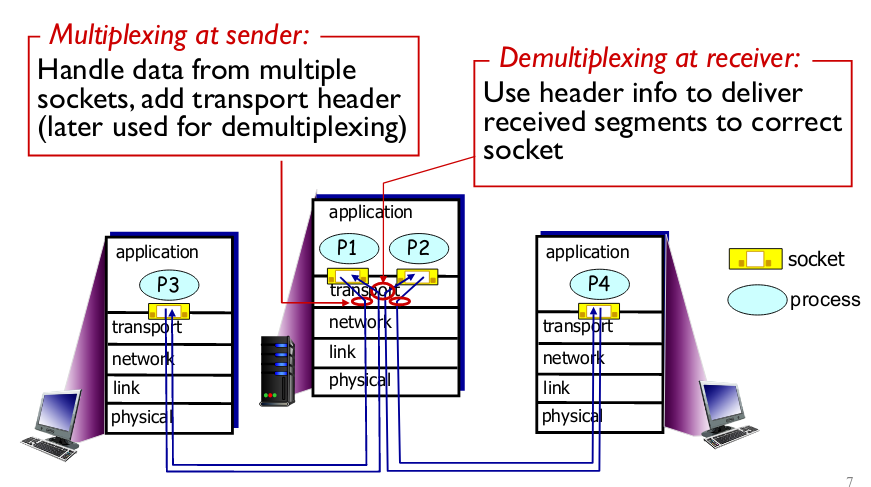
\includegraphics[scale=0.7]{multiplexing}
\end{center}
\begin{important}[Groups of data]
In the network layer it is called a packet\\
In the transport layer it is called a segment
\end{important}
\begin{itemize}
	\item Host receives IP datagrams
	\item Each datagram has source IP address, destination IP address
	\item Each datagram carries one transport-layer segment
	\item Each segment has source, destination port number
	\item Host uses IP addresses and port numbers to direct segment to appropriate socket
	\item Each socket has a unique identifier
\end{itemize}
\begin{center}
	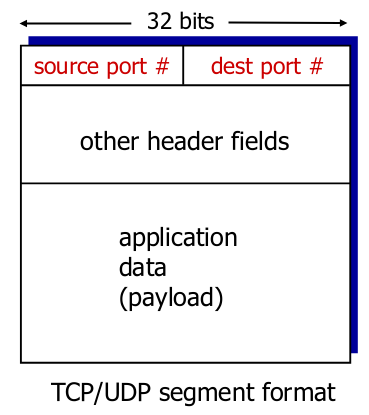
\includegraphics[scale=0.7]{segment}
\end{center}
\subsection{Connectionless multiplexing and demultiplexing}
\begin{itemize}
	\item All sockets have host-local port \#
	\item Assigned automatically, or via \texttt{bind()}
	\item \texttt{serverSocket,bind((ip, port))}
	\item When host receives UDP segment:
	\begin{itemize}
		\item Checks destination port \# in segment
		\item Directs UDP segment to socket with that port \#
	\end{itemize}
\end{itemize}
If two UDP segments have different source IP addresses and/or source port numbers but same dest IP and port \#, they will be directed to same process via same process via same socket as dest
\begin{center}
	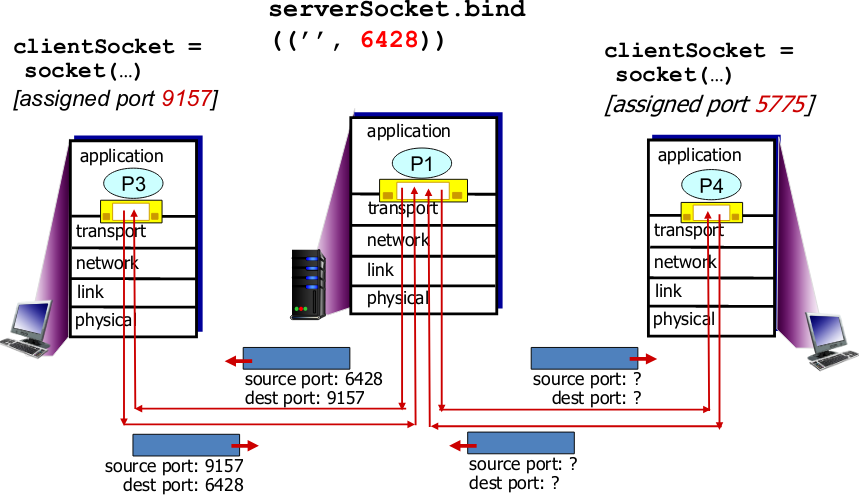
\includegraphics[scale=0.7]{demultiplexing}
\end{center}
\subsection{Connection-oriented multiplexing and demultiplexing}
TCP socket identified by 4-tuple
\begin{itemize}
	\item Source IP address
	\item Source port number
	\item Destination IP address
	\item Destination port number
\end{itemize}
Demux: receiver used all four values to direct segment to appropriate socket\\
Server host may support many simultaneous TCP sockets:
\begin{itemize}
	\item Each socket identified by its own 4-tuple
	\item Two arriving TCP segments with different source IP/ \#Port will be directed to two different sockets
\end{itemize}
\begin{center}
	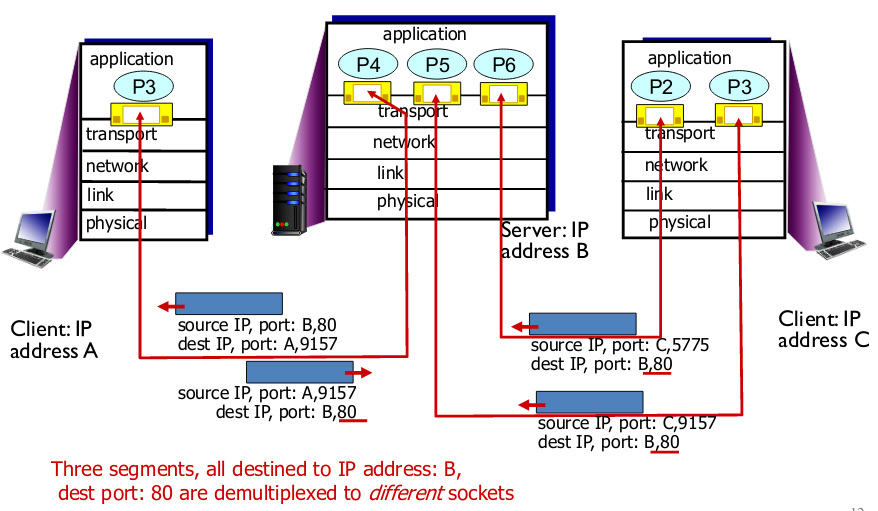
\includegraphics[scale=0.7]{connection}
\end{center}
\begin{important}[TCP Sockets]
With TCP we have a different socket for each connection	
\end{important}
\section{Connectionless transport: UDP}
\begin{itemize}
	\item "No frills", "bare bones" internet transport protocol
	\item "Best effort" service, UDP segments may be
	\begin{itemize}
		\item Lost
		\item Delivered out-of-order to app
	\end{itemize}
	\item Connectionless:
	\begin{itemize}
		\item No handshaking between sender/receiver
		\item Each UDP segment handled independently of others
	\end{itemize}
	\item UDP use:
	\begin{itemize}
		\item Streaming multimedia apps (loss tolerant, rate sensitive)
	\end{itemize}
	\item Reliable transfer over UDP
	\begin{itemize}
		\item Add reliability at application layer
		\item Application-specific error recovery
	\end{itemize}
\end{itemize}
\subsection{Segment Header}
\begin{center}
	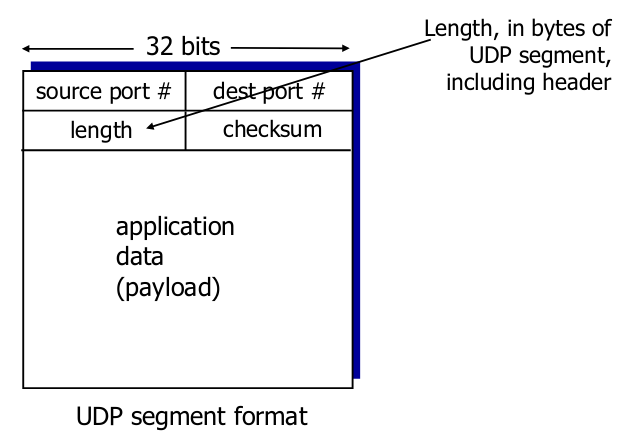
\includegraphics[scale=0.7]{udp}
\end{center}
\section{Principles of reliable data transfer}
\begin{center}
	\includegraphics[scale=0.7]{"reliable data transfer"}
\end{center}
Note that reliable data transfer protocol is not a standard, it is just for us to look at academically
\begin{center}
	\includegraphics[scale=0.7]{"reliable data transfer1"}
\end{center}

\end{document}